%
% ---------- header -----------------------------------------------------------
%
% project       kaneton
%
% license       kaneton
%
% file          /home/mycure/kaneton/view/paper/design/design.tex
%
% created       julien quintard   [wed may 16 18:26:51 2007]
% updated       julien quintard   [thu jun 14 14:35:13 2007]
%

%
% ---------- setup ------------------------------------------------------------
%

%
% path
%

\def\path{../..}

%
% template
%

%
% ---------- header -----------------------------------------------------------
%
% project       kaneton
%
% license       kaneton
%
% file          /home/mycure/kaneton/view/template/paper.tex
%
% created       julien quintard   [wed may 16 18:17:37 2007]
% updated       julien quintard   [fri oct  5 07:00:45 2007]
%

%
% class
%

\documentclass[10pt,a4wide]{article}

%
% packages
%

\usepackage[english]{babel}
\usepackage[T1]{fontenc}
\usepackage{a4wide}
\usepackage{fancyheadings}
\usepackage{multicol}
\usepackage{indentfirst}
\usepackage{graphicx}
\usepackage{color}
\usepackage{xcolor}
\usepackage{verbatim}
\usepackage{aeguill}

\pagestyle{fancy}

\setlength{\footrulewidth}{0.3pt}
\setlength{\parindent}{0.3cm}
\setlength{\parskip}{2ex plus 0.5ex minus 0.2ex}

%
% logos
%

\newcommand{\logos}
  {
    \begin{center}
      
\includegraphics[scale=0.8]{\path/logo/kaneton.pdf}
    \end{center}
  }

%
% prototype
%

\newcommand\prototype[2]{
  \begin{tabular}{p{0.2cm}p{13.8cm}}
  & #1
  \end{tabular}

  \begin{tabular}{p{1cm}p{13cm}}
  & #2
  \end{tabular}}

%
% verbatim stuff
%

\definecolor{verbatimcolor}{rgb}{0.00,0.40,0.00}

\makeatletter

\renewcommand{\verbatim@font}
  {\ttfamily\footnotesize\selectfont}

\def\verbatim@processline{
  {\color{verbatimcolor}\the\verbatim@line}\par
}

\makeatother

%
% header
%

\rhead{}
\rfoot{\scriptsize{The kaneton microkernel project}}

\date{\scriptsize{\today}}


%
% header
%

\lhead{\scriptsize{The kaneton microkernel design}}

%
% title
%

\title{The kaneton microkernel project \\
       \scriptsize{http://www.kaneton.org}}

%
% authors
%

\author{\small{Julien Quintard}}

%
% document
%

\begin{document}

%
% title
%

\maketitle

%
% ---------- abstract ---------------------------------------------------------
%

\begin{abstract}

This paper describes the design of the kaneton microkernel.
This system was designed to be ported on many architectures without being
intrusive. The main goal of this system is to be understandable
by everyone interested in operating systems internals. To do so, the kaneton
design and implementation are very elegant and very easy to understand.
The kaneton microkernel includes modern distributed paradigms
leading to a powerful, secure, flexible and reliable microkernel based
operating system.

\end{abstract}

%
% --------- text --------------------------------------------------------------
%

\begin{multicols}{2}

%
% the kaneton history
%

\section{The kaneton history}

kaneton originated in Paris, France as an educational project in operating
systems. The project was primarily designed by two students Julien Quintard
and Jean-Pascal Billaud although many other people also contributed to
the design and especially to the implementation.

Having recently contributed to the development of a microkernel based
operating system called LSE/OS, the two students decided to begin the
design and development of an operating system with a more powerful design
and able to share resources on a large network. Nevertheless, the goal of
this project remains to be an educational one. For this reason, the
designers focused on the simplicity of the design and the implementation.

The two students wanted to break some well-known kinds of computer sciences
rules. Indeed, for example, many computer scientists consider that a
project documentation is in fact its source code. Many low-level system
programmers also consider that the kernel boot source code and more
generally the kernel source code cannot be understandable by everyone
because too hardware-dependent and then messy.

People tried, in kaneton, to write documentation for every part of the
project. Moreover people tried to build a microkernel understandable
by everyone interested in operating systems internals via an elegant
and coherent design but also implementation.

%
% the kaneton goals
%

\section{The kaneton goals}

Many research projects in operating systems started with an existing system.
For the kaneton microkernel project, people decided to design a totally
new system. Indeed, the LSE/OS project was not portable enough, so the
kaneton people decided to design a new kernel from scratch with a
special interest for the portability.

The kaneton microkernel was developed in a very specific way, to build
a pedagogical project, with the clearest possible design to become an
all easy-to-understand project including source code, design etc.

The kaneton microkernel will become the base of a distributed operating
system. For this reason, the kaneton microkernel was designed to fit
the distributed operating system requirements. For example, the kaneton
microkernel includes modern distributed concepts like capabilities
which open many interesting ways to security features and flexibility.

The kaneton source code is extremely clear and heavily commented which
make the project easily maintainable.

Needless to say the kaneton project being a microkernel is extremely small
and provides only fundamental functionalities. Nonetheless, the kaneton
microkernel design obviously implies a core bigger than many other
microkernels.

Finally, the kaneton microkernel will be able to run
UNIX{\scriptsize \copyright} programs via a POSIX emulation library.

%
% the kaneton architecture
%

\section{The kaneton architecture}

Before describing the kaneton microkernel internals, it is useful first to
outline the kind of hardware for which the system was designed.

The kaneton microkernel has been designed to deal with multiple architectures
and heterogeneous systems.

Since the kaneton portability system was designed not to be intrusive, the
microkernel has no precise requirement.

Although the kaneton microkernel design does not seem to fit embedded
systems, the kaneton core can be parameterise to use for example specific
fixed-size data structures. The same notice goes for other specific
architectures.

%
% the kaneton microkernel
%

\section{The kaneton microkernel}

A microkernel based operating system is composed of two parts:
a \textbf{microkernel} which runs on every processor machine of the system
and a collection of \textbf{servers} that provides most of traditional
operating system functionalities: drivers, file servers etc.

The microkernel has four primary functionalities to provide:

\begin{enumerate}
  \item
    Communication.
  \item
    Memory management.
  \item
    Process management.
  \item
    I/O.
\end{enumerate}

Although the microkernel architecture is already modular, the kaneton
microkernel is also subdivided into managers. This subdivision leads to
a better understanding since each manager provides an interface to control
a precise type of kaneton object.

For example, there exists an address space manager, a task manager,
a thread manager etc. So the reader interested in understanding how
the threads are implemented in kaneton just has to read the source code
in relation with the thread manager, nothing more.

Moreover, each manager interface's function naming follows a precise
nomenclature. This nomenclature leads to a better coherence of the whole
microkernel.

This paper will now describe microkernel's components to understand how
the kaneton microkernel provides communication, memory management, process
management etc.

%
% communication
%

\subsection{Communication}

The kaneton microkernel and more generally the distributed operating
system uses messages to communicate with everything.

Keep in mind that the kaneton project must be as simple as possible to be
understood by students.

To unify communications via messages, the microkernel translates every event
into a message. For example, when an interrupt is received by the kernel
interrupt handler, a message is built and forwarded to the server dedicated
to this interrupt. So, each server just has to take care of how to receive
messages and how to reply to them.

Note that no group communication is provided by the microkernel. Indeed, the
group communication concept is inherent to the distributed operating system.
Therefore, the group communication will not be explained in this paper.

Moreover, unlike UNIX-like operating systems, the kaneton microkernel does
not use signals. Indeed, the goal of the kaneton microkernel is not to
be as fast as a monolithic type kernel like Linux.

The kaneton project focuses on genericity, coherency, abstractions etc.

Finally, the kaneton message passing interface was designed based on
well-known parallel and distributed programming libraries like MPI. From
this fact, the kaneton microkernel directly includes concurrent
programming facilities.

%
% memory
%

\subsection{Memory}

The memory model of the kaneton microkernel is very simple.

Each address space of the system is composed of segments and regions.

A \textbf{segment} consists in a linear sequence of physical addresses.
A segment describes one area of physical memory including the
first address, the last but also some properties like the owner of this
segment, the permissions: execution, read, write etc. and some
extra attributes. Segments can be accessed via mappings or directly via
the segment manager interface provided by the kaneton microkernel.

A \textbf{region} consists in a linear sequence of virtual addresses.
A region has no properties and is only used to map a valid segment.
Using a region in the virtual memory will reference the segment's data
it maps.

An \textbf{address space} is a list of memory locations. In the kaneton
microkernel, an address space includes the list of the segments and regions.
So, an address space describes the available process' memory.

Like the entire system, the kaneton memory model is based on little objects
which are linked to build more complex objects. An address space is composed
of segments and regions. This model implies that a program is allowed to
manage its entire memory itself, its physical memory like its virtual one.

Note that this paper does not explain the memory algorithm used to manage
physical memory areas. Indeed, the memory manager uses the set manager
to store its data. For this reason, the segment manager can easily change
the algorithm used for storing its data.

By \textit{easily} we mean that a single line has to be modified in the
source code.

For more information about the set manager, please refer to its
specific section.

%
% objects and protections
%

\subsection{Objects And Protections}

First of all, every kaneton object is identified by a unique identifier
and manipulated over the microkernel with a capability.

As said before, many kaneton objects are built by linking objects
together.

The figure below illustrates the hierarchy of the kaneton objects
and the kaneton microkernel itself.

\begin{center}
  
\includegraphics[scale=0.35]{figures/kaneton.pdf}
\end{center}

Recall that the kaneton microkernel was designed to fit distributed
operating systems requirements.

This means that, contrary to classical operating systems, the microkernel
has to provide distributed-specific features. First, any reserved
objects must be secured over the network to avoid security issues.

Indeed, for example, on a classical operating system, when a user process
asks the kernel for opening a file, the kernel just returns a file descriptor.
In this context, there is no need to secure the file descriptor since
this descriptor is private to the process' address space which asked for it.

In a distributed operating system, the returned file descriptor may
be transfered over the network to the caller. Then, in this context,
an attacker could intercept the file descriptor and use it to access
the file.

So, a distributed system needs to protect the objects over the network.

The second distributed-specific feature the microkernel has to provide
is to allow a process which holds a resource, to grant access to another
process, with equal or less rights, to its resource.

This feature open many ways in managing fine-grained security over
the distributed operating system.

The kaneton designers then decided to use capabilites to handle these
two distributed-specific features in relation with the security.

A \textbf{capability} provides an easy way to allow a task of the
system to access a privileged object via a very simple cryptographic
technique.

Although this concept was introduced for the distributed operating systems
needs, the kaneton designers decided to exploit the capabilities' properties.

Indeed, the capabilities permit a task to restrict the permissions
of an owned capability and then to distribute this restricted capability
to other tasks. Then, these tasks get the right to access the privileged
object but this right is limited by the capability's permissions the
capability's owner previously set.

This concept is very interesting, even in classical operating systems,
because it allows tasks to handle the security on the objects they own.

To illustrate this concept, consider a program which allocates a segment of
physical memory. Then it decides to allow another process to only read
this segment. It will so generate a less privileged capability and give
it to the other process. Therefore, the second process will be able to read
the segment but not to write it.

A common capability format includes the object identifier, the permissions
of the capability on the object listing the allowed operations, a check field
ensuring security and other specific fields like for example the location
of the service, a lifetime etc.

The figure below illustrates the capability generic format used in the Amoeba
distributed operating sytem, this capability format being used by every
server of the distributed system.

\begin{center}
  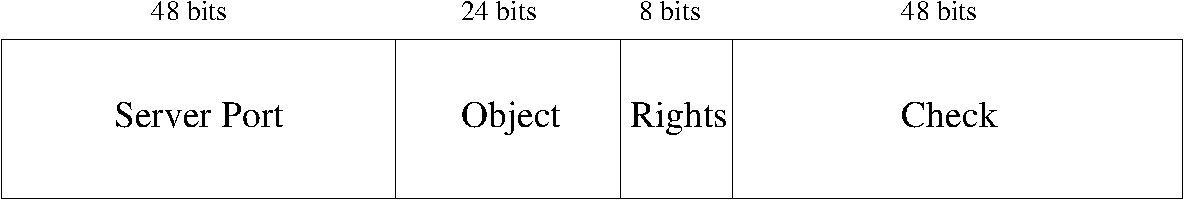
\includegraphics[scale=0.35]{figures/capability.pdf}
\end{center}

Unlike many distributed systems, the kaneton microkernel based
distributed operating system will use specific and specialised capabilites,
rather than generic capabilities, to increase scalability.

Consider a modern file system with billions of inodes; this file system
certainly wants to build capabilities with a 64-bit identifier.

Consider now another service, for example a printer service, listing
every printer of the system. This service certainly wants to use 16-bit
identifier in its capabilities because there will certainly never be more
than 65000 printers on this system.

Each server is different so each server needs its own capability format.

The use of specific and specialised capabilites forces the programs to ask
the servers to generate new capabilites, unlike other systems. Indeed,
the other systems generally use generic capabilites to permit programs to
generate capabilities by themselves. This was not the kaneton designers'
choice and the result is more scalable capabilites but a performance loss
in capability generation.

Note that libraries for each capability type manipulation could also have
been provided but this was not the kaneton designers' choice either.

Moreover, using this scheme permits servers to use the cryptographic
algorithm they want.

Note that the capability generation does not often happen so the performance
loss is not dramatic. Moreover, a capability can be generated and used
by many other tasks because capabilites are generally used to restrict
permissions. A capability is not unique to its user, so a program can
generate a capability and distribute it to many other programs giving
them the same permissions.

To conclude, this system is performant in a normal use but can become
very slow if a program has to generate many different capabilities, this
case being seldom.

The use of specific capabilities also allows servers to create capabilities,
for example, without identifier or with extra permission fields or with
maximum security using for example a 128-bit check field.

Note that the use of the check field does not guarantee security over the
distributed system. For this reason, the kaneton microkernel based
distributed operating system can evolve with three security policies:

\begin{enumerate}
  \item
    \textbf{No security}: with this policy, the security field of the
    capabilities is not used. No cryptography is used on the system
    to guarantee security.
  \item
    \textbf{Local security}: with it, the capabilities are protected from
    malicious programs and users using the check field. So, while there
    is no network message passing of capabilites, the system can be
    considered as safe.
  \item
    \textbf{Global security}: with this security policy, the distributed
    operating system is safe. Every capability is protected with its check
    field but in addition each message on the network is protected by
    cryptographic algorithms.
\end{enumerate}

%
% set
%

\subsection{Set}

The kaneton microkernel internally uses a set manager which organises data
for other kernel managers. The entire microkernel is based on the sets.

Using this manager leads to a very elegant and maintenable source code. For
example the task manager uses the set manager to store every task of the
system. Additionnaly, each task contains a set composed of the threads of
this task etc.

Such a system provides an easy way to store data without effort. The task
manager for example does not care about how to store data.

Furthermore, it is possible to optimise the code where it needs to be. In
this case, it will be useful to optimise the data structures in the set
manager and \textit{not} in every manager using such a data structure like
other systems do.

Indeed, the other operating systems generally use pointers to link kernel
structures together and implicitly form sets. Such a source code is human
unreadable and leads to many programming confusions and errors.

kaneton being an educational microkernel project, kaneton people wanted
to use the simplest design possible.

The set manager provides many different data structures like double
linked-list, stack, pipe, array, b+-tree etc. In addition, the set
manager can be extended without affecting the other managers using it.

The set manager also provides tools like \textbf{iterators} to easily and
quickly go through sets object.

The set manager's interface is generic, independently of the underlying set
implementation. From this fact, a manager using a set can easily modify
the set implementation used just by modifying a word in the set
object reservation line, the other set manager function calls do not
need to be modified.

The set manager is a key concept of kaneton because the whole kaneton
core source code uses it leading to a very coherent and understandable
source code.

The set manager manages what are called \textbf{set objects}. These set
objects are actually used to store data. Note that, the set objects are
also stored in a set object.

Indeed, the set manager uses itself to store the set objects. The special
set object which stores the set objects is called the \textbf{set container}.

The figure below illustrates the sets interconnections.

\end{multicols}

\begin{center}
  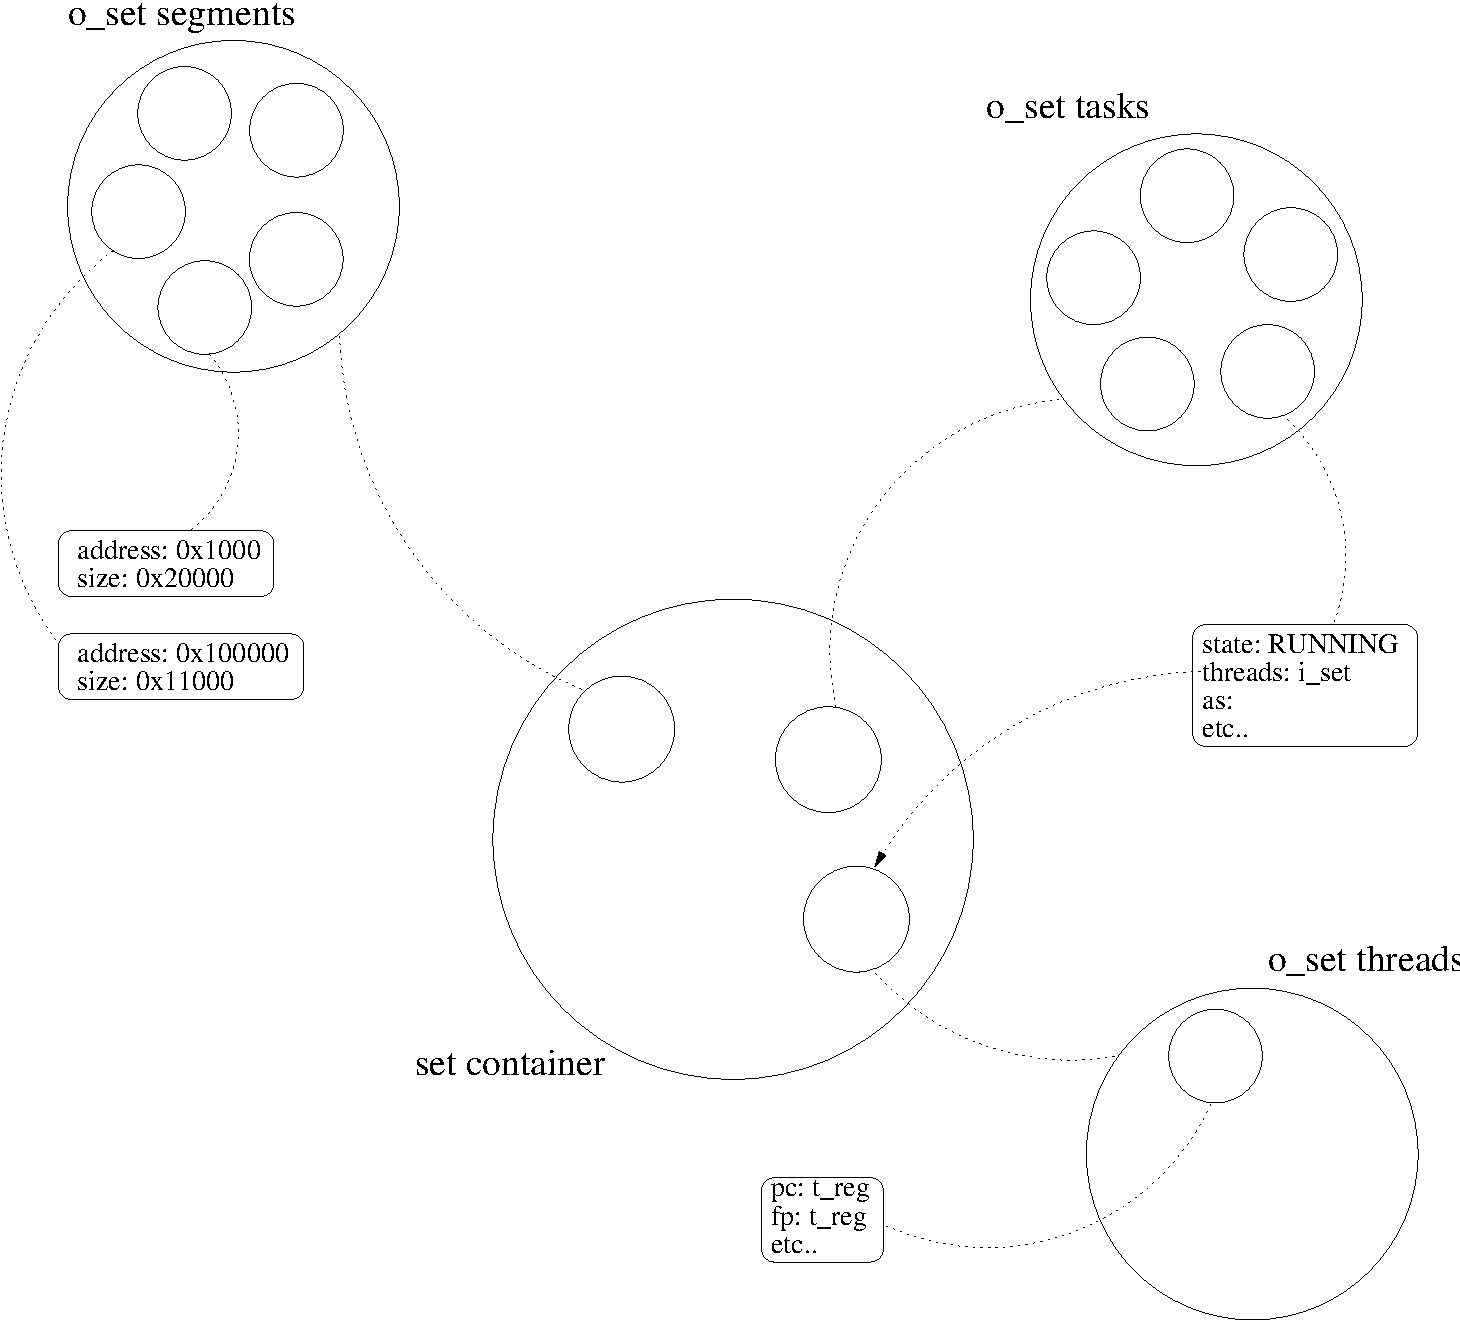
\includegraphics[scale=0.5]{figures/sets.pdf}
\end{center}

\begin{multicols}{2}

The reader should notice on this figure that the set container holds
three set objects. One of this set is used to hold task objects.

Task objects are basically composed of memory and threads. For this
reason, each task contains a set of threads.

The figure illustrates the complex organisations of set interconnections.

Although this scheme seems complex, the implementation does not
suffer from this complexity. The resulting effect is a concentration
of the kernel complexity in a single point: the set manager.

The rest of the kaneton core implementation is so extremely simple.

%
% process
%

\subsection{Process}

The kaneton microkernel uses a specific nomenclature which is different
from other operating systems.

The system is composed of five different entities in relation with execution.

A \textbf{module} represents a passive execution entity in main memory.
Indeed, a module does not run and has no execution context. The modules are
managed by the module service to reside in main memory the time it is
necessary. For example a very used program like \textit{/bin/ls} will
certainly become an important module due to its frequent use.

Fundamental system's drivers and services are persistent modules because
they would be used in the case of a crash to restart the crashed service
without any dependency to the hard drive device driver for example.

A \textbf{program} is the lowest privileged task on the system.
The common user programs are the well-known UNIX{\scriptsize \copyright}
programs like \textit{/bin/ls}, \textit{/bin/wc}, \textit{/usr/bin/cc} etc.
A program is a task with no privilege. All it can do is compute some things,
manage data and send messages to more privileged processes.

A \textbf{service} is a server which provides a so-called service. A service
waits for messages, performs a task, and returns the result of the service
replying the caller.

A \textbf{driver} is a service which can communicate with hardware devices.
So, the I/O operations are reserved to tasks which are at least a driver.

Finally, a \textbf{core} is a kind of super-driver in which it provides
many services and communicates with hardware devices. Moreover, it is
the only task able to modify every system's internal data structure.

In typical microkernel, every task can only be called by less or equal
privileged tasks. In kaneton, we decided to break this rule because we found
it too restrictive. In fact the cores are allowed to send asynchronous
messages. Without this exception, the microkernel is not able to forward
messages, so hardware and software communications are not possible.

The kaneton microkernel does not have processes in the
UNIX{\scriptsize \copyright} sens of the term. Indeed, the kaneton
microkernel manages tasks. A \textbf{task} is a non-active entity because
a task is never scheduled. A task, in the kaneton terms, is an abstraction
which describes an execution environment, a context. Each task has an
address space describing its useable memory and one or more threads.
A task with only an address space and one thread is essentially identical
to a UNIX{\scriptsize \copyright} process. The term \textbf{process} is
sometimes used in the kaneton documentation to describe a kaneton task.

The \textbf{threads} are the active entities because they are the one
scheduled. Such a thread belongs to a single task, has a set of registers,
a program counter and finally a stack. Needless to say that the kaneton
microkernel handles threads as kernel threads.

Each task has three important properties: a class, a behaviour and a priority.

The \textbf{class} is chosen at the task creation time. This property
informs the kernel about the nature of the task, its role on the system.
In addition, this class will implicitly determine the rights of the task
on the system. The different classes are \textit{core}, \textit{driver},
\textit{service}, \textit{program}. On many architectures, the core, driver
and service classes will have the same hardware system priority.
Nevertheless, few architectures provide different hardware system privileges
like the Intel 32-bit Architecture.

The \textbf{behaviour} specifies the kernel, the type of the task from the
scheduler point of view. The different values for the behaviour are
\textit{core}, \textit{realtime}, \textit{interactive}, \textit{timesharing}
and \textit{backgroud}. Each behaviour defines a range of priorities for the
task.

The \textbf{priority} is a value included in the range defined by the
task's behaviour. Any thread of a task can update the priority of its
task in this range, modifying the task priority from the scheduler
point of view.

With these properties, a user can create a task very reactive setting an
appropriate behaviour and then updating its priority to adjust its quantum.
This mechanism gives the programs many possibilities and permits them to
choose their execution context.

The threads also have an important property: a priority.

Each thread of a task can set its own priority in the range $[10, 250[$.
Therefore, a thread can set itself an higher priority than the other
threads of its task. The resulting effect is a thread having a longer quantum
so better interactivity. Once again, this mechanism gives more liberty to the
programs.

%
% statistics
%

\subsection{Statistics}

The kaneton microkernel includes a statistics manager which performs
runtime statistics on managers.

Indeed, this manager collects information on functions used by each manager
including the number of calls, the number of errors and the time passed
in each function.

Whenever a function is called and returns, the statistics manager is notified
and then updates its data structures.

Through this statistics manager kaneton developers are able to optimise
the critical managers and functions.

Needless to say that the set manager is part of the critical managers since
the whole kaneton core is based on it.

%
% machine dependent
%

\section{The kaneton portability system}

This section describes the specific kaneton portability system.

The portability can be implemented through two different ways in kernels.

The first way consists in the development of an entire part, functionality
of the kernel, for a specific architecture. For example, let's consider the
memory manager. The memory manager source file will be totally redeveloped
for each architecture on which the kernel will be ported. This system leads
to source code redundancy but also to the optimum performances since
it is possible to use every external architecture facilities to optimise
the kernel execution on this architecture.

The second way consists in the design of an architecture interface defining
the common architecture operations like \textit{tlb\_flush()},
\textit{install\_page\_directory()} etc. This system is better than the
first from the redundancy point of view. Nonetheless, optimisations are more
difficult to implement. Furthermore, it is still possible for an architecture
not to fit in this interface. Then, the kernel could not be ported on
this architecture.

The kaneton designers were not satisfied by these two solutions and so
decided to adapt the second solution to the kaneton microkernel design.

The kaneton solution consists in a kind of extension of the second solution
in which no interface is designed. Rather, every time a kaneton object is
created, modified or destroyed, the machine-dependent source code is called
to permit it to perform some operations on the object or on everything else.

This pseudo-interface is better than the previous ugly and static one.
Despite this improvement, there still exists the possibility of an
architecture not fitting in this portability system.

kaneton people decided to use this system because it provides the most
dynamic, moldable portability system. This system is experimental but
seems to be functional. Theoritically, this system is optimum because
there is no redundancy and there are no constraints for the
machine-dependent source code.

Moreover, this portability system is not intrusive, meaning that there
is no need to modify a single line of the machine-independent source code
to port kaneton on another microprocessor architecture.

The kaneton portability system was developed, in its earliest version,
using c-preprocessor's macros.

%
% implementation
%

\section{Implementation}

The kaneton microkernel project was created in a pedagogical way.

Indeed, the kaneton authors provide many materials for the kaneton
microkernel development including complete documentation and assignments.

Moreover, documentation on specific architectures are also provided
to help students in a precise implementation.

In addition, the kaneton authors are developing a microkernel reference
as a basis for future development in distributed systems.

This reference implementation was written using the C language and
modern tools.

The current kaneton microkernel reference implementation is being
ported on Intel 32-bit architectures and MIPS 32-bit and 64-bit architectures.

%
% conclusion
%

\section{Conclusion}

The kaneton microkernel is based on a simple paradigm which allows
programmers to manage memory and execution context as they want to.

A special interest was ported on parallel and distributed programming
providing complete primitives to manage priorities on many levels:
thread, task etc. but also via a complete message passing interface.

The set manager is used to make the kernel source code very elegant
and then understandable by everyone including students. Moreover, the
data structure management is centralised in a unique point limitating
the bugs and increasing the possible optimisations.

The kaneton portability system was designed to perfectly fit the
kaneton microkernel requirements. Indeed, this portability system
is not intrusive and allows kaneton to be ported on many different
architectures.

Finally, the kaneton microkernel uses modern concepts like
capabilities which open many ways to new security management but
also increase the reliability and flexibility.

For more information on the kaneton microkernel project, please refer
to the official kaneton website
  \footnote{http://www.kaneton.org}.

%
% acknowledgments
%

\section{Acknowledgments}

To the kaneton people especially C\'edric Aubouy, Matthieu Bucchianeri,
Enguerrand Raymond and Renaud Voltz.

\end{multicols}

\end{document}
